
\chapter{Gebäudeübersichten}

\section{Theresienstr. -- Mathebau}

\begin{center}
\bf Erdgeschoss \hspace{0.5\textwidth} 1. Stock

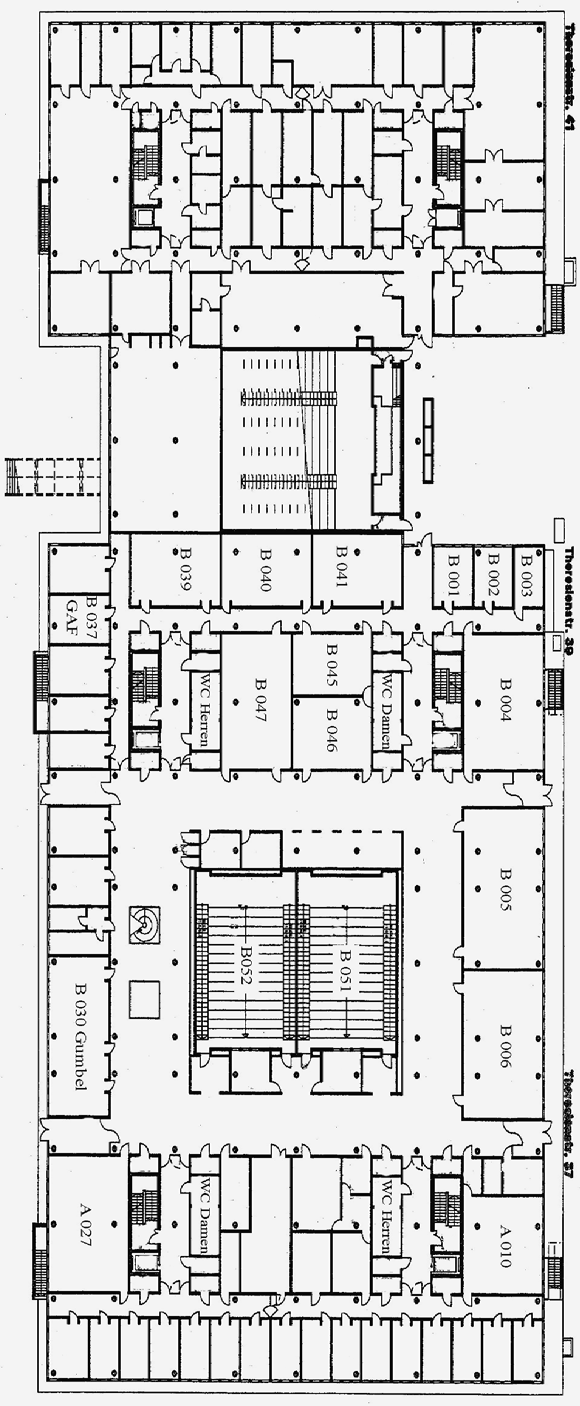
\includegraphics[width=0.49\textwidth]{theresien1.png}
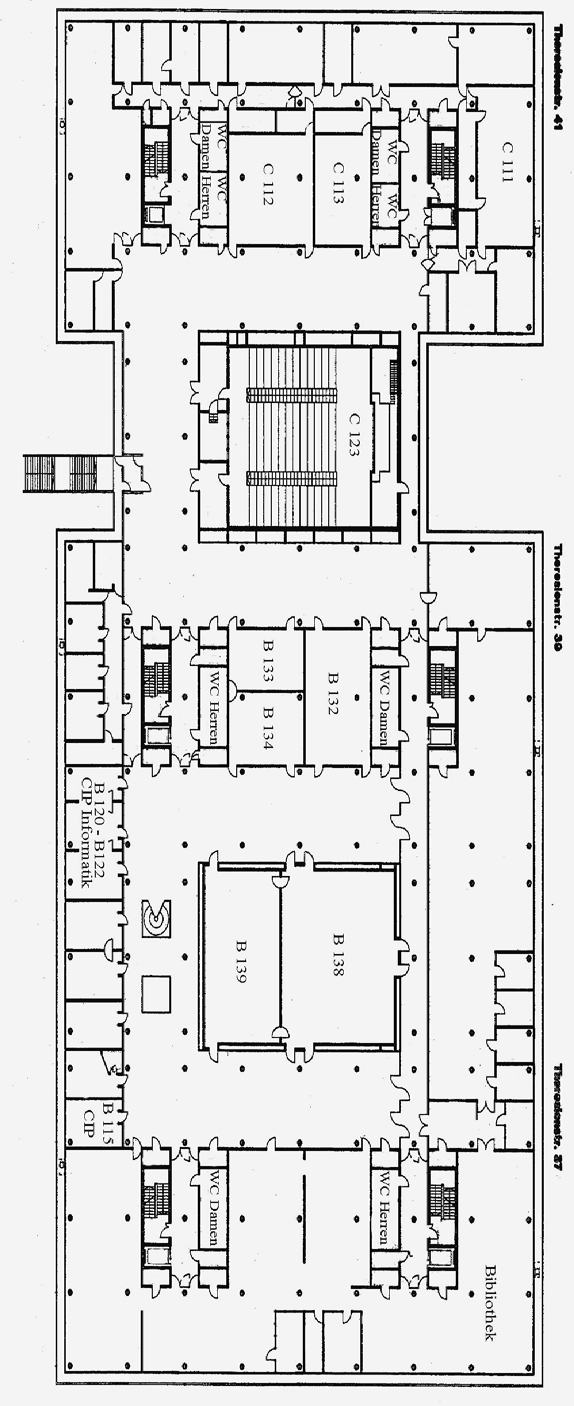
\includegraphics[width=0.49\textwidth]{theresien2.png}


\section{Oettingenstraße -- Erdgeschoss}

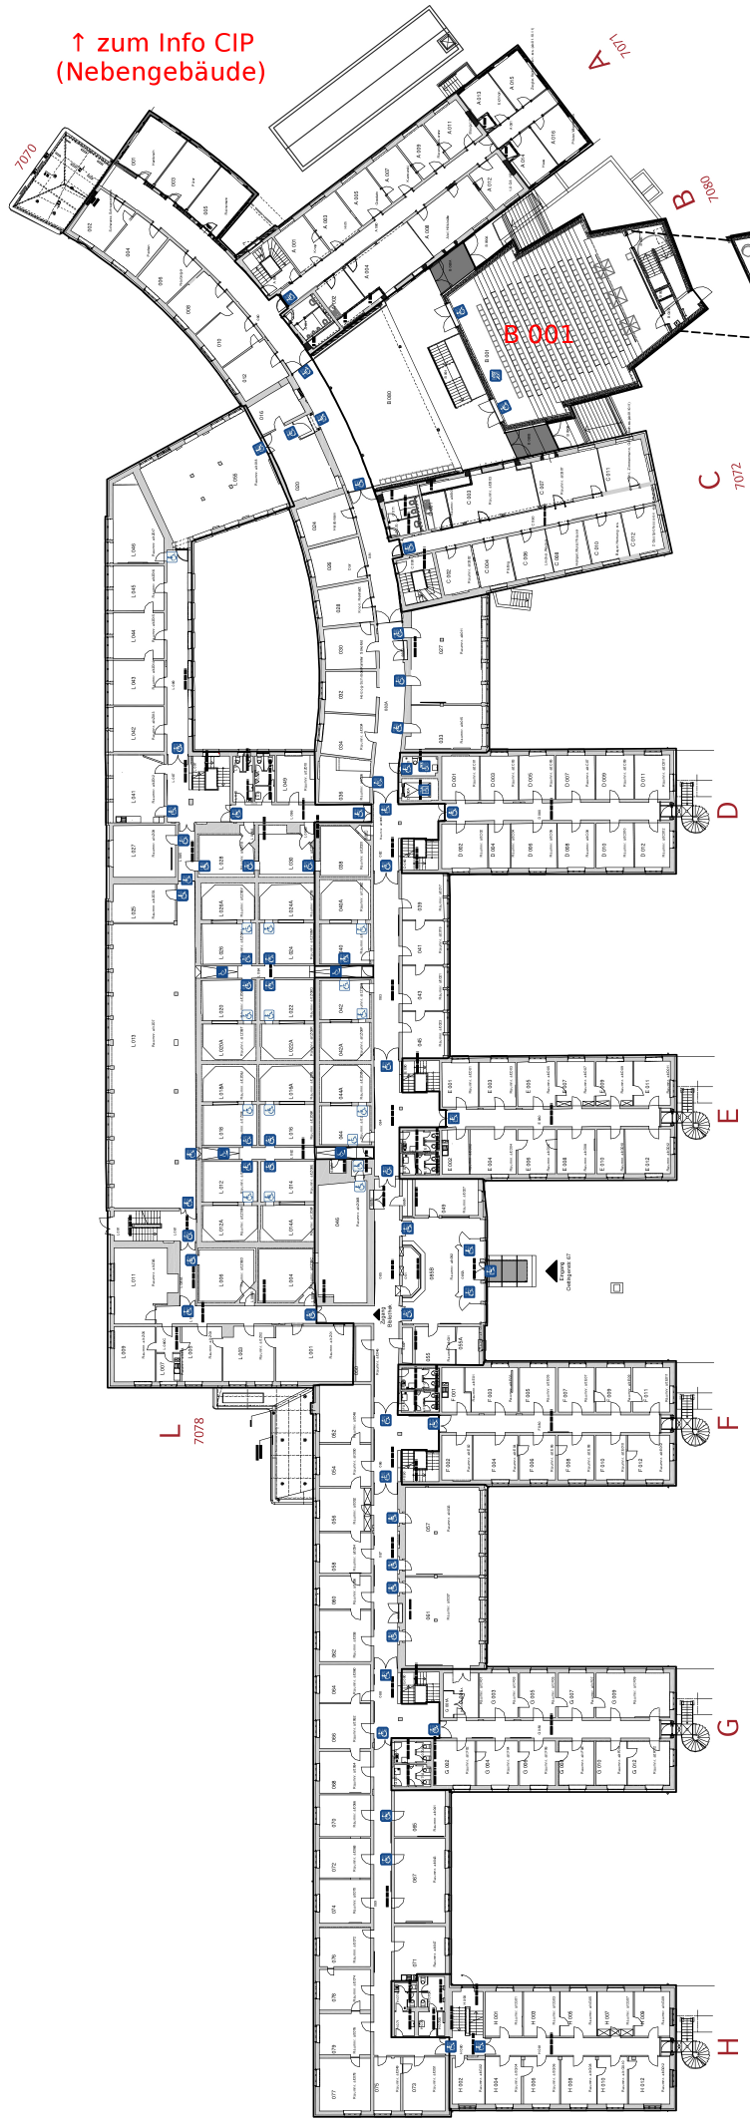
\includegraphics[height=0.9\textheight]{oettingen.png}

\section{Schellingstr. 4 -- Physik}


\includegraphics[width=0.5\textwidth]{schelling.png}

\section{Hauptgebäude}

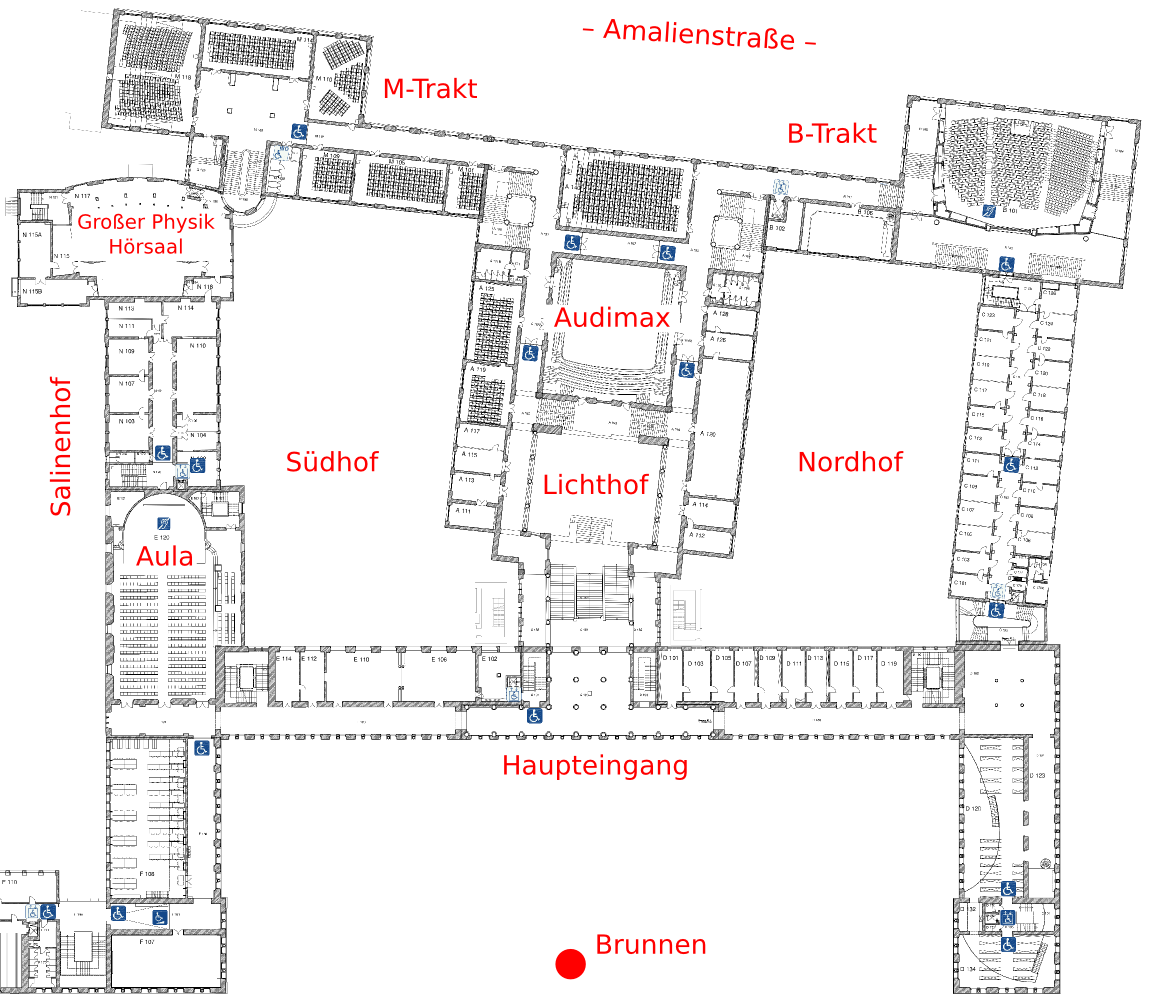
\includegraphics[height=0.6\textheight]{hauptgeb.png}

\end{center}

\begin{multicols}{2}
\setlength{\parindent}{0pt}
